\documentclass[10pt]{article}
\usepackage[margin=1.0in]{geometry}
\usepackage{graphicx}
\usepackage{float}
\usepackage[nottoc,numbib]{tocbibind}
%\usepackage[backend=biber,sorting=none]{biblatex}
\usepackage{siunitx}
\usepackage{pgfgantt}
\usepackage{tabularx}
\usepackage{rotating}
%\usepackage{xcolor, colortbl}
\usepackage{enumitem}
\usepackage{setspace}
\usepackage{wrapfig}
\usepackage[acronyms,toc,nonumberlist]{glossaries}
\usepackage{booktabs}
\usepackage[hidelinks]{hyperref}
\usepackage{blindtext}
\usepackage{setspace}
\usepackage{footnote}

\newcommand{\tabitem}{~~\llap{\textbullet}~~}
\makesavenoteenv{tabular}
\renewcommand{\acronymname}{Nomenclature}
%\addbibresource{final_report.bib}
\makenoidxglossaries
\glsnoexpandfields
\loadglsentries{gloss.tex}

\title{
  AERSP 401B \\
  Spacecraft Design \\
  Executive Summary \\
  Reusable Lunar Surface Access Vehicle \\
}

\date{}

\begin{document}
\doublespacing

\clearpage\maketitle
\thispagestyle{empty}

\begin{center}
  
\includegraphics{SeleneSupplyLogo}\hspace*{\fill}\\  
  TEAM SELENE SUPPLY \\
  \begin{tabular}{l r}
    Team Leader: & Nicholas \textsc{Pytel} \\
    Gracie \textsc{Ryan} & Dominick \textsc{Allen} \\
    Robert \textsc{Bond} & Tyler \textsc{Meehan} \\
    Adalberto \textsc{Morales} & Michael \textsc{Croydon} \\
  \end{tabular}

  \hspace{1cm} \newline
  \hspace{1cm} \newline
  Instructor: Dr. David \textsc{Spencer} \\
  November 30, 2018
\end{center}

\newpage
\setcounter{page}{1}

\newpage

\section{Motivation/mission purpose}

The reusable Lunar Surface Access Vehicle (LSAV) has the primary
purpose of providing transportation means between the Lunar Gateway
and the lunar surface utilizing transfers from the Near Rectilinear
Halo Orbit of the gateway. This mission will provide support for
future Lunar missions and base operations by carrying both crew and
cargo too and from the surface of the moon. The mission will prove the
viability of the Lunar Gateway as a platform for future missions

\section{Mission Objectives  requirements, constraints}

In order to support lunar missions, the LSAV must satisfy the
following requirements: Must transport either crew or cargo to the
lunar surface Capable of transporting a maximum of 15 metric tons to
the surface and 10 metric tons from the surface Capable of supporting
a crew of up to four people for the duration of the mission and 24
hours on the surface.  Capable of landing anywhere (within reason) on
the lunar surface Must be reusable

These requirements are satisfied by the following design decisions:

The LSAV will be propelled by a methane/LOx raptor engine and will be
refuelable at the lunar gateway The LSAV will support a cargo bay and
crew capsule capable of supporting the above noted requirements. The
cargo bay will provide storage space and also support a
loading/unloading crane from moving cargo to/from the surface.  The
life support system will provide moderate radiation shielding and a
breathable atmosphere during crewed operations. The Life support
system will use polycarbonate shielding as well as Lithium based CO2
scrubbers for crew support. Oxygen and water will be provided from a
small storage system separate from the propulsion system.  The
electrical system will provide power via solar panels and battery
banks. The battery banks will be capable of supplying a minimum of 36
hours of energy which will allow for operations on non illuminated
portions of the moon.  The structure will support a landing leg
assembly which will allow for landing on surfaces up to a slope of 12
degrees and free of large debris.  The LSAV will be supported by the
SpaceX ‘Starship’ launch vehicle until it reaches the Lunar Gateway
after which it will be self operating.  Refueling and resupply will
occur at the Lunar Gateway and will be supported by other NASA
missions outside the scope of this mission.

\begin{figure}[H]
  \centering
  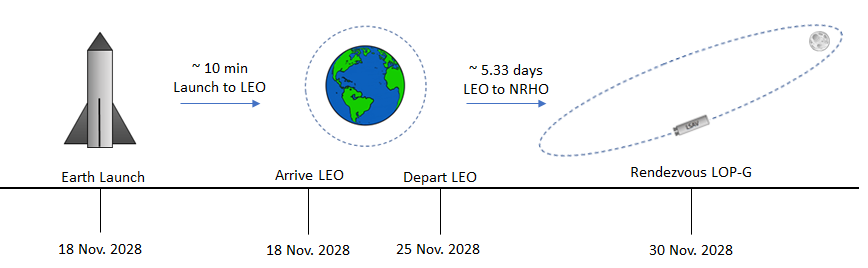
\includegraphics[width=0.9\textwidth]{toon1}
  \caption{Earth launch to LOP-G timeline}
  \label{fig:toon1}
\end{figure}

\begin{figure}[H]
  \centering
  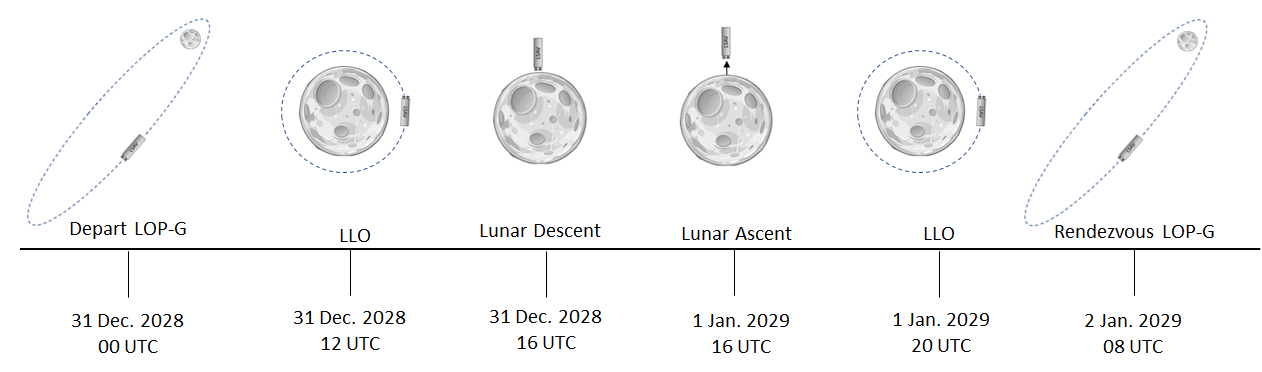
\includegraphics[width=0.9\textwidth]{toon2}
  \caption{LOP-G to lunar surface cycle timeline}
  \label{fig:toon2}
\end{figure}

\begin{table}
  \centering
  \caption{foo}
  \label{table:foo}
  \begin{tabular}{ccc}
    Mass (metric ton) & Power (kWhr) & Cost (USD) \\
    50 (230 wet) & 1388 & 8.1 Billion \\
  \end{tabular}
\end{table}

\section{Requirements / Derived  requirements / Sequence
  of events}

LSAV Launches from Cape Canaveral and is injected into LEO System
checkouts occur while Starship is refueled over the course of a week
Starship transfers the LSAV from LEO to NRHO and gets in close
proximity to the station Starship separates, the LSAV propulses itself
and rendezvous with the gateway.  LSAV is refueled and final system
checks occur over the course of 3 weeks Crew arrives at the lunar
gateway and the LSAV is loaded with first mission cargo LSAV departs
gateway and lands on surface Surface mission completes, LSAV launches
from surface with crew and return cargo LSAV rendezvous with lunar
gateway, crew and cargo depart and vehicles is refueled.  System
checks occur over the course of 2 weeks and any maintenance required
is completed.  Vehicle launches for next mission.  Cycle repeats for
either 30 missions or 5 years System architecture, cartoon Mass, Cost,
Power stuff Subsystems

\textbf{Propulsion} - The tank pressurization system will use gaseous methane
and oxygen to feed the liquid propellent to the raptor engine. This
system will reduce the cost per mission by omitting the need for
helium tanks.

\textbf{ECLSS} - The crew will be housed in the front of the spacecraft with a 6
cm polyethylene radiation shield lining the walls. The 60 gallon water
supply tank will be place in the nose cone to also partially protect
against radiation.

\textbf{Ground Control} - Mission control will be shared between the Lunar
Gateway and the Lyndon B. Johnson Space Center. The Lunar Gateway will
be the primary SOCC and POCC.

\textbf{Communication} - The communication system has been changed to use only
S/X-Band antennae. UHF was originally going to be used for
communications between the LSAV and the Lunar Gateway, but this ended
up being too low frequency for the 80,000 km distance between the
Gateway and the LSAV. The same set of two S-Band antennae will be used
to receive communications from the Near Earth Network (NEN) and to
transmit and receive data to and from the Lunar Gateway. Additionally,
a half meter parabolic X-band antenna will be used to transmit data to
the NEN.

The power requirements for the communications system has changed with
the removal of the UHF antennae as well. When transmitting data to the
NEN will require 40 W of power for a data rate of 5 mbps, and
transmitting to the Lunar Gateway will require 24 W of power for a
data rate of 512 kbps. Additionally, the LSAV will be capable of
receiving 128 kbps of data on both the X-band and S-band antennae,
while consuming a total of 10 W of power.

The 5 mbps of data transmitted to the NEN will be sufficient for
mission data, such as life support and possibly video feeds. When the
LSAV is not in view of the NEN, the 512 kbps of data transmitted to
the Lunar Gateway should be sufficient for basic mission data and
telemetry. The 128 kbps of data the LSAV can receive will be
sufficient for any commands that need to be sent. Note that the data
rate for receiving data from the Lunar Gateway assumes a range of
80,000 km, which is the absolute farthest the two will be from each
other while in operation. At a closer range of approximate 1000 km,
the LSAV will easily be capable of receiving upwards of 10 mbps from
the Gateway.

Finally, BPSK was chosen as the modulation scheme for all
communications. BPSK is chosen because practically all NEN ground
stations are capable of using it. BPSK requires higher \(\frac{E_b}{N_o}\)
compared to other modulation schemes, but its universality makes up
for this.

\textbf{Guidance, Navigation and Control} - The attitude of the LSAV
will be adjusted by a set of MR-107V engines using
hydrazine. Attitude, position, and velocity will be determined by sun
sensors, star sensors, and IMUs that are Kalman filtered by radiation
hardened RAD5545 computers. During docking, LIDAR will be used to fine
tune the approach to the International Berthing and Docking Mechanism
on the LSAV.

\textbf{Power} - The four battery banks will have their own charge
controller/monitors capable of independent operation. This will
increase the safety and reliability of the electrical system while
also providing a more stable output to the rest of the system.


The solar panels will be capable of gimbaling to allow the power input
into the system to be throttled and to match the required power. This
will mitigate the thermal burden on the thermal system by mitigating
wasted input power.

\textbf{Launch Vehicle}- SpaceX BFR \& Starship will be used to carry the LSAV
to an equatorial parking orbit

Payload This system must be capable of transferring 15/10 mT of cargo
to and from the surface of the moon. Cargo is stored in the upper
portion of the LSAV so a system of cranes and sliding platforms will
be used to move this cargo. An internal crane will load cargo onto a
sliding platform which will transfer the cargo to the exterior of the
craft. Finally, an external crane will move the cargo from the
platform down to the surface of the moon, an approximately 10 m
descent, where astronauts or autonomous vehicles will be prepared to
move the cargo from the loading/unloading area.

One danger is that loading/unloading cargo from the center of mass of
the ship creates the possibility of the ship tipping over. To prevent
this, the crane will extend less than 5 m from the center of mass of
the ship, which will be within the base created by the landing
legs. As an additional precaution, the cargo will be divided into
parcels small enough to keep any tipping moment within a safe
margin. This safe margin will be based on the moments of inertia of
the ship at landing.


\newpage
\section{Appendix}

\begin{table}
  \centering
  \caption{Reasonable assumptions were made for the Gateway's power
    and communications capabilities.}
  \label{table:linkbudgetlsav}
  \begin{tabular}{lrr}
    {} & LSAV to Gateway &Gateway to LSAV \\

    Transmit Power (P)&24 W&45W \\

    Line  Loss \((L_l)\)&-1 dB&-1 dB \\
    Transmit Gain \((G_t)\)&25 dB&35 dB \\
    Space Loss \((L_s)\)&-197.6 dB&-197.6 dB \\
    Path Loss \((L_a)\)&0 dB&0 dB \\
    Receiving Gain \((G_r)\)&30 dB&30 dB \\
    System Temperature Noise \((T_s)\)&27.9 dB&27.9 dB \\
    Data Rate (R)&512 kbps&128 kbps \\
    Implementation Loss \((L_i)\)&-2 dB&-2 dB \\
    Estimated \(\frac{E_b}{N_o}\)&11.9 dB&30.6 dB \\
    Required \(\frac{E_b}{N_o}\)&8.5 dB&10.5 dB \\
    Link Margin&3.4 dB&20.1 dB \\

  \end{tabular}
\end{table}

\begin{tabular}{lrr}
  &LSAV to NEN&NEN to LSAV \\
  Transmit Power (P)&40 W&200 W \\
  Line  Loss \((L_l)\)&-1 dB&-1 dB \\
  Net Transmit Gain* \((G_t)\)&29.5 dB&44.8 dB \\
  Space Loss \((L_s)\)&-224.9 dB&-212.9 dB \\
  Path Loss \((L_a)\)&-1 dB&-1 dB \\
  Receiving Gain \((G_r)\)&61.7 dB&30 dB \\
  System Temperature Noise \((T_s)\)&27.9 dB&27.9 dB \\
  Data Rate (R)&5 mbps&128 kbps \\
  Implementation Loss \((L_i)\)&-2 dB&-2 dB \\
  Estimated \(\frac{E_b}{N_o}\)&12 dB&30.6 dB \\
  Required \(\frac{E_b}{N_o}\)&8.5 dB&10 dB \\
  Link Margin&3.5 dB&20.6 dB \\
\end{tabular}


Mass, power tables, link budget Subsystem costs Supplementary
subsystem info

Power

The battery bank controllers will each be capable of independent
control and will be interfaced with each other and the main LSAV
control system. This will allow fine tuning of power input/output of
each battery bank based on proximity to the load. It will also allow
for fast countermeasures to take place in the event of a critical
battery failure by keeping the control system local to the individual
battery bank.

The solar cell arrays will be capable of adjusting their solar flux
exposure by changing their angle relative to the solar radiation
source. This will mitigate the use of radiative power dissipation
systems in the event that the system has fully charged batteries and
is generating more power than the LSAV requires. In addition to
mitigating solar flux input, it can also be used to maximize flux
input when solar flux is not normal to the cell arrays. This will
allow maximum energy harvesting which will allow for more power usage
during missions (if needed).

Structures and Mechanical Systems



\section{Motivation}
  % \input{abstract.tex}
\blindtext

\section{Mission Objectives}
\blindtext

\section{Requirements}
\blindtext


\end{document}